\documentclass{VUMIFPSkursinis}
\usepackage{algorithmicx}
\usepackage{algorithm}
\usepackage{algpseudocode}
\usepackage{amsfonts}
\usepackage{amsmath}
\usepackage{bm}
\usepackage{caption}
\usepackage{color}
\usepackage{float}
\usepackage{graphicx}
\usepackage{listings}
\usepackage{subfig}
\usepackage{wrapfig}
\usepackage{enumitem}
\usepackage{multirow}
\usepackage[utf8]{inputenc}
%\usepackage{enumerate}

%PAKEISTA, tarpai tarp sąrašo elementų
\setitemize{noitemsep,topsep=0pt,parsep=0pt,partopsep=0pt}
\setenumerate{noitemsep,topsep=0pt,parsep=0pt,partopsep=0pt}

% Titulinio aprašas
\university{Vilniaus universitetas}
\faculty{Matematikos ir informatikos fakultetas}
\department{Programų sistemos}
\papertype{Laboratorinis darbas}
\title{Kelionių į Mėnulį maršrutų planavimo programos „Poon“ prototipo panaudojamumo testavimas}
\status{3 kurso 5 grupės studentai}
\author{Gabrielė Žielytė}
\secondauthor {Daumantas Šimkus}
\thirdauthor {Nedas Valentinovičius}
\titleineng{}

\date{Vilnius – \the\year, Galutinė versija}

% Nustatymai
\setmainfont{Palemonas}   % Pakeisti teksto šriftą į Palemonas (turi būti įdiegtas sistemoje)
\bibliography{bibliografija}

\begin{document}
	
% PAKEISTA	
\maketitle

%TURINYS
\thispagestyle{empty}
\tableofcontents

\sectionnonumnocontent{Anotacija}
Šiame dokumente aprašomas bilietų pirkimo kelionėms į mėnulį telefoninės programos „Poon“ prototipo panaudojamumo testavimas. Kiekvienas komandos narys prisidėjo prie prototipo kūrimo naudodami „JustInMind“ prototipavimo priemonę. Studentų, dirbusių prie šio projekto, kontaktai:
\begin{itemize}
\item Gabrielė Žielytė - gabriele.zielyte@mif.stud.vu.lt. 
\item Daumantas Šimkus - daumantas.simkus@mif.stud.vu.lt. 
\item Nedas Valentinovičius - nedas.valentinovicius@mif.stud.vu.lt.
\end{itemize}
\thispagestyle{empty}

\cleardoublepage\pagenumbering{arabic}
\setcounter{page}{4}

\section{Santrauka}
Šiame dokumente bus patekti „Poon“ prototipo testavimo rezultatai. Prototipą testavo kruopščiai atrinkti penki asmenys, kurie atitinka panaudojamomo scenarijus. Juos sudaro statistikos departamento darbuotojas, neregys, senjoras, žmogus perkantis kelionės bilietus tik sau bei žmogus, bilietus perkantis sau ir draugams. Testavimą vertino „Poon“ trijų kūrėjų komanda, testuotojams davusi prieeigą prie programos ir prižiūrėjusi visą testavimo procesą.

\section{Įvadas}
Kelionių į Mėnulį bilietų pirkimo programos „Poon“ prototipas kurtas pagal apibrėžtus maketus pasinaudojant nemokama prototipavimo priemone „JustInMind“. Ši programa turi integruota apmokymo sistemą, kuri greitai ir nesudėtingai leido kurti prototipą, atsižvelgiant į vartotojų poreikius.


\section{Testavimo aprašas}
\subsection{Testuojamos užduotys}
\begin{itemize}
\item Pirkti bilietą(us) \\
	\textbf{Kriterijai:}
	\begin{itemize}
	\item Sistema neparodo lango, jog ne visi laukai užpildyti
	\item Pasirinktas skrydis tik į vieną pusę arba į abi
	\item Pasirinktas išvykimo miestas
	\item Pasirinktas atvykimo miestas
	\item Pasirinktos išvykimo atvykimo datos
	\item Pasirinktas teisingas keleivių skaičius
	\item Rastas patraukliausias skrydis(-džiai)
	\item Pasirinta teisingai keleivių lytis
	\item Suvesti keleivių vardai ir pavardės
	\item Pasirinktos sėdėjimo vietos
	\item Paspaustas mygtukas „Tvirtinti“ duomenis
	\item Neprireikė vertintojo pagalbos
	\item Atlikta greičiau nei per 2min
	\end{itemize}
	\textbf{Sekmės matas:} Pasiektas bilietų apmokėjimo langas \\

\item Sumokėti už kelionės bilietą(us)  \\
	\textbf{Kriterijai:}
	\begin{itemize}
	\item Sistema neparodo lango, jog ne visi laukai užpildyti
	\item Neprireikė vertintojo pagalbos
	\item Pasirinktas mokėjimo būdas
	\end{itemize}
	\textbf{Sekmės matas:} Sistema parodo langą, jog bilietai sėkmingai nupirkti \\

\item Parsisiųsti statistiką  \\
	\textbf{Kriterijai:}
	\begin{itemize}
	\item Nunaviguota į statistikos langą
	\item Pasirinkta kompanija
	\item Pasirinktas duomenų formatas
	\item Neprireikė vertintojo pagalbos
	\item Užduotis atlikta greičiau nei per 1min
	\end{itemize}
	\textbf{Sekmės matas:} Sistema parodo langą, jog statistika sėkmingai parsisiųsta \\

\item Pakeisti nustatymus  \\
	\textbf{Kriterijai:}
	\begin{itemize}
	\item Nunaviguota į nustatymų langą
	\item Pakeistas nustatymas
	\item Neprireikė vertintojo pagalbos
	\item Atlikta per mažiau nei minutę
	\end{itemize}
	\textbf{Sekmės matas:} Pakeitus nustatymus sėkmingai grįžta į pradinį langą \\
\end{itemize}

\subsection{Metodas}
Testavimui buvo pasirinktas metodas kai vertintojas viso testavimo proceso metu stebi testuotoją ir seka jo progresą, o iškilus bėdai suteikia pagalbos pasižymėdamas, jog testavimas neįvyko nepriekaištingai. Testuotojas buvo supažindintas su užduotimis kurias jis turi atlikti.

\subsection{Aplinka}
Testavimas vyksta testuotojui natūralioje aplinkoje t. y. jo namuose, darbe ar miesto kavinėje. Testuotojui buvo duotas išmanusis telefonas su iOS operacine sistema, kurioje yra įrašyta  „Poon“ prototipavimo programa.

\subsection{Dalyviai}

Dalyvių charakteristikų lentelė, sukurta remiantis klausimynų atsakymais.
\begin{figure}[H]
    \centering
    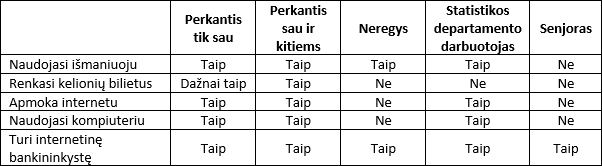
\includegraphics[scale=1]{img/lentele.png}
    \caption{Dalyvių charakteristikos}
    \label{img:dch}
\end{figure}

\section{Testavimo rezultatai}
\subsubsection{Užduočių vykdymo rezultatai}
Dalyvių rezultatai sugrupuoti pagal užduotis:
	\begin{itemize}
	\item 1-oji užduotis \\
Visi testuotojai atliko užduotis.
	\item 2-oji užduotis \\
Visi testuotojai atliko užduotis.
	\item 3-oji užduotis \\
Visi testuotojai atliko užduotis.
	\item 4-oji užduotis \\
Visi testuotojai atliko užduotis. Neregiui prireikė pagalbos ieškant neregiams skirto nustatymo, bet užduotį įvykdė.
	\end{itemize}
\subsubsection{Dalyvių komentarai}
Komentarai sugruputi pagal užduotis:
	\begin{itemize}
	\item 1-oji užduotis \\
	Visi testuotojai patenkinti užduotimi.
	\item 2-oji užduotis \\
	Visi testuotojai patenkinti užduotimi.
	\item 3-oji užduotis \\
	Visi testuotojai patenkinti užduotimi.
	\item 4-oji užduotis \\
Visi testuotojai patenkinti užduotimi.
	\end{itemize}

\section{Rekomendacijos}
Rekomendacijų skyriuje analizuojamas rastų defektų sunkumas ir dažnis, skaičiuojami prioritetai, pateikiami siūlomi defektų sprendimai. \\ \\
Neregys rekomenduoja iškelti neregystės nustatymų mygtuką į pagrindinį langą, tačiau jis užduotį atliko. Statistikos departamento darbuotojas siūlo praturtinti statistika, nes dėl statistikos jis nesinaudotų „Poon“ programa.

\section{Priedai}
Visi priedai atskiruose dokumentuose.
\subsection{Klausimynai}
\subsection{Dalyvių rezultatų lentelės}
\subsection{Dalyvio sutikimo dalyvauti testavime raštas}


\printbibliography[heading=bibintoc, title=Šaltiniai]  % Šaltinių sąraše nurodoma panaudota
\end{document}
